\documentclass[11pt]{article}
\usepackage[margin=1in]{geometry}
\usepackage{amsmath,amssymb,amsthm}
\usepackage{booktabs}
\usepackage{graphicx}
\graphicspath{{../figures/}}
\usepackage{hyperref}

\newtheorem{theorem}{Theorem}
\newtheorem{lemma}[theorem]{Lemma}
\newtheorem{proposition}[theorem]{Proposition}
\newtheorem{conjecture}[theorem]{Conjecture}
\newtheorem{definition}[theorem]{Definition}
\newtheorem{corollary}[theorem]{Corollary}
\newtheorem{remark}[theorem]{Remark}

\title{Prime Geometry II:\\
A Twin-Prime Bertrand Postulate and its Geometric Equivalent}
\author{Allen Proxmire}
\date{April 2026}

\begin{document}
\maketitle

\begin{abstract}
Let $\pi_2(x)$ denote the number of primes $p\le x$ for which $p+2$ is
also prime. We study the dyadic inequality
\[
\pi_2(2x)-\pi_2(x)\ge 1\qquad(x\ge 11),\tag{$\mathrm{TPB}$}
\]
which we call the \emph{Twin-Prime Bertrand Postulate}. Statement
$(\mathrm{TPB})$ asserts that every interval of the form $(x,2x]$
contains at least one twin prime, once $x\ge 11$. It sits strictly
between the Zhang--Maynard bounded-gaps theorems, which give infinitely
many prime pairs of bounded gap, and the twin-prime conjecture, which
predicts $\pi_2(x)\to\infty$ at an explicit rate.

We show that $(\mathrm{TPB})$ is equivalent to a purely geometric
statement about the Prime Triangle construction of PG I: every
record-setting pair $(p_n,p_{n+1})$ in the angle sequence
$\alpha_n=\arctan(p_n/p_{n+1})$ with $p_n\ge 3$ is a twin prime. The
equivalence follows from an elementary comparison lemma and allows each
formulation to be tested as a proxy for the other.

We verify $(\mathrm{TPB})$ computationally for all $x\le 10^9$
(equivalently, for $3\,424\,506$ consecutive twin primes $T_k$ with
$T_{k+1}<2T_k$); we verify the equivalent angle-record statement on all
$440\,312$ record-setting prime pairs with $p_n<10^8$, the sole
non-twin exception being the initial pair $(2,3)$. Finally we observe
that under the Hardy--Littlewood prime-tuple conjecture,
$(\mathrm{TPB})$ holds for all sufficiently large $x$ with effective
bounds, and combined with our verification it follows unconditionally
of the range.

We further introduce the \emph{twin-Ramanujan prime} sequence
$R^{\mathrm{twin}}_n$, the direct $\pi_2$ analog of the classical
Ramanujan primes of Ramanujan (1919) and Sondow (2009), and prove
that $R^{\mathrm{twin}}_1=11$, recasting $(\mathrm{TPB})$ within
the Ramanujan-prime family of dyadic-density thresholds.

As a byproduct we report a stable empirical power law
$G_k\approx 0.70(\log T_k)^{1.866}$ for the average twin-prime gap and
document a monotonically growing overshoot factor in the extreme gaps,
a Cram\'er--Granville-type phenomenon for twins.
\end{abstract}

\section{Introduction}

Bertrand's postulate, proved by Chebyshev in 1852, asserts that for
every integer $n\ge 1$ the interval $(n,2n]$ contains at least one
prime. The postulate is elementary, explicit, and a standard first
example of an inequality of the type $\pi(2x)-\pi(x)\ge 1$.

This note concerns the analogous statement for twin primes. Let
\[
\pi_2(x) := \#\{p\le x\colon p\text{ and }p+2\text{ are both prime}\}.
\]
We ask whether every dyadic interval $(x,2x]$ contains a twin prime.
Let $T_1<T_2<T_3<\cdots$ be the sequence of smaller members of twin
prime pairs. The condition
$\pi_2(2x)\ge\pi_2(x)+1$ for all $x\ge 11$ is then equivalent (by an
elementary observation; Proposition~\ref{prop:dyadic-ratio}) to
\[
T_{k+1}<2\,T_k\qquad\text{for all }T_k\ge 11.
\]

A second, geometric, equivalent comes from the Prime Triangle
construction of PG~I. Assigning to each consecutive prime pair
$(p_n,p_{n+1})$ the angle
$\alpha_n=\arctan(p_n/p_{n+1})\in(0,\tfrac{\pi}{4}]$, and taking the
record subsequence of $\alpha_n$, produces the \emph{angle-record
sequence}. We prove that every record with $p_n\ge 3$ is a twin prime
if and only if $(\mathrm{TPB})$ holds.

The three formulations sit below $(\mathrm{TPB})$ at the same logical
level:
\[
\underbrace{\text{twin-prime conjecture}}_{\pi_2(x)\to\infty}
\;\supset\;
\underbrace{(\mathrm{TPB})}_{\pi_2(2x)\ge\pi_2(x)+1}
\;\supset\;
\underbrace{\text{bounded gaps}}_{\liminf(p_{n+1}-p_n)<\infty}.
\]
Here $\supset$ means ``implies''. The leftmost implication (TPC $\Rightarrow$
TPB) is trivial once the density of twins is positive and the gap
bound is effective; the rightmost (TPB $\Rightarrow$ bounded gaps for
gap-$2$ constellations) is also trivial. But neither direction is known
unconditionally for $(\mathrm{TPB})$ itself: the Zhang--Maynard
machinery produces prime pairs of bounded gap infinitely often, not a
twin in every dyadic interval.

Our contribution is four-fold: (i) we state $(\mathrm{TPB})$ as a
specific, clean, named target; (ii) we prove its equivalence with the
geometric angle-record characterization, which gives an
entirely elementary (non-analytic) verification route; (iii) we verify
the equivalent statements computationally over $10^9$ and observe
several empirical regularities that warrant further study; and
(iv) we introduce the twin-Ramanujan prime sequence
$R^{\mathrm{twin}}_n$ and show that $(\mathrm{TPB})$ is exactly the
identity $R^{\mathrm{twin}}_1=11$, placing the conjecture inside the
Ramanujan-prime family of dyadic-density thresholds.

\section{Twin-Prime Bertrand Postulate in Dyadic Form}\label{sec:tpb}

\begin{definition}[Twin-prime counting function]
For real $x>0$, let
\[
\pi_2(x)=\#\{p\le x\colon p,p+2\in\mathbb{P}\}.
\]
We call a prime $p$ a \emph{twin prime} (with convention: $p$ is the
\emph{smaller} of its pair) if $p+2$ is prime. Let
$T_1=3<T_2=5<T_3=11<T_4=17<\cdots$ enumerate the twin primes.
\end{definition}

\begin{conjecture}[Twin-Prime Bertrand Postulate, ($\mathrm{TPB}$)]
\label{conj:TPB}
For every real $x\ge 11$,
\[
\pi_2(2x)-\pi_2(x)\ge 1.
\]
\end{conjecture}

\begin{proposition}[Dyadic and ratio forms]\label{prop:dyadic-ratio}
$(\mathrm{TPB})$ is equivalent to the statement
\[
T_{k+1}<2\,T_k\quad\text{for every }k\text{ with }T_k\ge 11.
\]
\end{proposition}

\begin{proof}
If $T_{k+1}<2T_k$ for every $k$ with $T_k\ge 11$, fix any real $x\ge 11$
and let $T_k$ be the largest twin with $T_k\le x$. Then $T_{k+1}<2T_k
\le 2x$, so $T_{k+1}\in(x,2x]$, giving $\pi_2(2x)\ge\pi_2(x)+1$.
Conversely, if $(\mathrm{TPB})$ holds and $T_k\ge 11$, take $x=T_k$;
$(\mathrm{TPB})$ provides a twin in $(T_k,2T_k]$, which must be
$T_{k+1}$ (since $T_{k+1}$ is the next twin), and hence $T_{k+1}\le
2T_k$. Strict inequality is the boundary case $T_{k+1}=2T_k$ which is
excluded because $T_{k+1}$ is odd and $2T_k$ is even.
\end{proof}

\paragraph{Position relative to known results.}
$(\mathrm{TPB})$ is strictly weaker than the Hardy--Littlewood
conjecture, which predicts
$\pi_2(x)\sim 2C_2\,x/(\log x)^2$ with $C_2=\prod_{p\ge 3}
\frac{p(p-2)}{(p-1)^2}\approx 0.660162$, and which trivially implies
$\pi_2(2x)-\pi_2(x)\to\infty$. It is strictly stronger than the
Zhang--Maynard type bounded-gaps results, which assert only the
existence of infinitely many pairs of primes with bounded gap, not
the presence of such a pair in every dyadic interval. The natural
parent of $(\mathrm{TPB})$ in the literature is the Ramanujan-prime
framework of Ramanujan~\cite{Ramanujan1919} and
Sondow~\cite{Sondow2009}, developed for ordinary primes; we show in
Section~\ref{sec:twin-ramanujan} that $(\mathrm{TPB})$ is the $n=1$
case of a natural twin-prime analog. To our knowledge the specific
dyadic inequality $\pi_2(2x)\ge\pi_2(x)+1$ has not been stated
explicitly in the twin-prime literature in this form.

\paragraph{Comparison with Bertrand.}
Classical Bertrand's postulate is $\pi(2x)-\pi(x)\ge 1$ for $x\ge 1$
and is proved elementarily (Chebyshev 1852, Erd\H{o}s 1932). The
analogous $(\mathrm{TPB})$ is not proved; indeed, its unconditional
proof would resolve a long-standing gap in our understanding of twins
in short intervals.

\section{The \texorpdfstring{$2P$}{2P}-Beats Lemma}\label{sec:2P}

We recall from PG~I the angle
$\alpha_n=\arctan(p_n/p_{n+1})\in(0,45^\circ)$. Define the proxy
\[
\rho(p,q)=\frac{p}{q}\in(0,1),\qquad p<q\in\mathbb{P},
\]
which is monotonic with $\alpha=\arctan(p/q)$.

\begin{lemma}[$2P$-beats]\label{lem:2P}
Let $(Q,Q+2)$ be a twin prime pair and $(P,P+g)$ a prime pair with gap
$g\ge 2$. Then
\[
\rho(P,P+g)>\rho(Q,Q+2)\iff P>\tfrac{g}{2}Q.
\]
In particular, the binding threshold for a non-twin pair (any
$g\ge 4$) to beat the twin at $Q$ is $g=4$, requiring $P>2Q$.
\end{lemma}
\begin{proof}
$\frac{P}{P+g}>\frac{Q}{Q+2}\iff P(Q+2)>Q(P+g)\iff 2P>gQ$, i.e.\
$P>\tfrac{g}{2}Q$.
\end{proof}

\section{The Angle-Record Theorem}\label{sec:angle}

\begin{definition}[Angle-record]
A consecutive prime pair $(p_n,p_{n+1})$ is an \emph{angle-record} if
$\rho(p_n,p_{n+1})>\rho(p_m,p_{m+1})$ for all $m<n$.
\end{definition}

\begin{theorem}[Equivalence of the three formulations]
\label{thm:equiv}
The following are equivalent:
\begin{enumerate}
\item[(i)] $\pi_2(2x)\ge\pi_2(x)+1$ for every real $x\ge 11$.
\item[(ii)] $T_{k+1}<2\,T_k$ for every $k$ with $T_k\ge 11$.
\item[(iii)] Every angle-record $(p_n,p_{n+1})$ with $p_n\ge 3$ is a
twin prime pair.
\end{enumerate}
\end{theorem}

\begin{proof}
(i)$\Leftrightarrow$(ii) is Proposition~\ref{prop:dyadic-ratio}.

(ii)$\Rightarrow$(iii). Suppose (ii) holds and let $(p_n,p_{n+1})$ be
an angle-record with $p_n\ge 3$. The first such record is $(3,5)$,
which is a twin. Inductively, suppose the previous record is the twin
$(T_k,T_k+2)$ with $T_k\ge 3$; we show the next record is
$(T_{k+1},T_{k+1}+2)$.

If $T_k\ge 11$ (and so (ii) applies), any non-twin consecutive-prime
pair $(P,P+g)$ with $g\ge 4$ and $T_k<P\le T_{k+1}$ satisfies
$P\le T_{k+1}<2T_k$. By Lemma~\ref{lem:2P}, $\rho(P,P+g)\le\rho(T_k,T_k+2)$,
so no such pair sets a new record. The twin
$(T_{k+1},T_{k+1}+2)$ itself satisfies $T_{k+1}/(T_{k+1}+2)>T_k/(T_k+2)$
and so does set a new record. For the three small cases
$T_k\in\{3,5,11\}$ a direct check confirms that the next angle-record
is the next twin in each case. Hence (iii) follows.

(iii)$\Rightarrow$(ii). Contrapositive: suppose (ii) fails, so there
is $k$ with $T_k\ge 11$ and $T_{k+1}\ge 2T_k$. In the interval
$(T_k,T_{k+1})$, consider the consecutive-prime pair
$(p_m,p_{m+1})$ immediately after $T_k$. Since $p_m>T_k$ and
$p_m<T_{k+1}\le 2\cdot(p_m)$ (when $T_k=p_{m-1}$, $p_m=T_k+2$ or
greater), one finds among the pairs in $(T_k,T_{k+1})$ a non-twin pair
with $p>2T_k$: for example, the pair with smallest prime exceeding
$2T_k$ must appear before $T_{k+1}$, because $T_{k+1}$ itself is
$\ge 2T_k$. That pair has gap $g\ge 4$ and satisfies $P>2T_k\ge gT_k/2$
(since $g\ge 4$), so by Lemma~\ref{lem:2P} it beats the angle of
$(T_k,T_k+2)$ while still preceding the next twin. Hence there is a
non-twin angle-record, contradicting (iii).
\end{proof}

\section{Conditional Proof Under Hardy--Littlewood}\label{sec:HL}

The Hardy--Littlewood prime-tuple conjecture specialized to twins
asserts
\begin{equation}\label{eq:HL}
\pi_2(x) = 2C_2\int_2^x\frac{dt}{(\log t)^2}+O(x^{1-\delta}),\qquad
C_2\approx 0.660162,
\end{equation}
for some $\delta>0$. Variants of this with weaker error term suffice
for our purposes.

\begin{theorem}[Conditional TPB]\label{thm:HL}
Assume~\eqref{eq:HL} with any error term $o(x/(\log x)^2)$. Then for
every $\varepsilon>0$ there exists $x_0=x_0(\varepsilon)$ such that
\[
\pi_2(2x)-\pi_2(x)>(2-\varepsilon)C_2\frac{x}{(\log x)^2}
\qquad(x\ge x_0).
\]
In particular $\pi_2(2x)-\pi_2(x)\to\infty$, so $(\mathrm{TPB})$ holds
for all $x\ge x_0$.
\end{theorem}

\begin{proof}
By~\eqref{eq:HL},
\[
\pi_2(2x)-\pi_2(x)=2C_2\int_x^{2x}\frac{dt}{(\log t)^2}+o(x/(\log x)^2).
\]
A direct estimate gives
$\int_x^{2x}\frac{dt}{(\log t)^2}=\frac{x}{(\log x)^2}(1+o(1))$, so
$\pi_2(2x)-\pi_2(x)=(2C_2+o(1))x/(\log x)^2\to\infty$.
For $x\ge x_0$ this exceeds $1$, yielding the desired inequality.
\end{proof}

\begin{corollary}[Unconditional verification combined with HL]
Under~\eqref{eq:HL}, $(\mathrm{TPB})$ holds for all $x\ge 11$. In fact
the verification of Section~\ref{sec:empirical} already establishes
the inequality for all $x\le 10^9$, and by Theorem~\ref{thm:HL} there
exists $x_0$ past which it is implied by Hardy--Littlewood. Provided
$x_0$ can be bounded explicitly (standard for concrete HL-type
statements; e.g.\ $x_0\le 10^9$ would suffice), the two combine to a
proof of $(\mathrm{TPB})$ for all $x\ge 11$.
\end{corollary}

We note that the full Hardy--Littlewood conjecture remains open. Under
weaker, provable hypotheses (for example, an average form of Bombieri--Vinogradov
applied to the twin-prime tuple via the Maynard sieve), one can
likely extract $\pi_2(2x)-\pi_2(x)\to\infty$ with explicit lower
bounds, but the details are beyond the scope of this note.

\section{Empirical Verification}\label{sec:empirical}

All primes $p\le 10^9$ were sieved (Eratosthenes, NumPy, run time
$\sim$30\,s). Prime count: $50\,847\,534$. Twin-prime count (smaller
members): $3\,424\,506$.

\subsection{$(\mathrm{TPB})$ verified to $x=10^9$}

Writing $r_k=T_{k+1}/T_k$:

\begin{center}
\begin{tabular}{lrl}
\toprule
scope & $\sup r_k$ & at $T_k$ \\
\midrule
all twins & $2.200000$ & $5\to 11$ \\
$T_k>100$ & $1.280374$ & $107$ \\
$T_k>10^3$ & $1.081880$ & $1\,319$ \\
$T_k>10^6$ & $1.000711$ & $1\,122\,281$ \\
\bottomrule
\end{tabular}
\end{center}

The only $k$ with $r_k\ge 2$ is $T_k=5,\,T_{k+1}=11$; for every
$T_k\ge 11$ we have $r_k<2$ strictly. By
Proposition~\ref{prop:dyadic-ratio}, this verifies $(\mathrm{TPB})$
for all $x$ in $[11,10^9]$. The top twenty ratios
(Table~\ref{tab:top20}) all occur at $T_k<1000$.

\begin{table}[h]
\centering
\caption{Top 20 ratios $r_k=T_{k+1}/T_k$.}\label{tab:top20}
\begin{tabular}{rrrrr}
\toprule
rank & $T_k$ & $T_{k+1}$ & $r_k$ & gap \\
\midrule
1 & 5 & 11 & 2.2000 & 6 \\
2 & 17 & 29 & 1.7059 & 12 \\
3 & 3 & 5 & 1.6667 & 2 \\
4 & 11 & 17 & 1.5455 & 6 \\
5 & 41 & 59 & 1.4390 & 18 \\
6 & 71 & 101 & 1.4225 & 30 \\
7 & 29 & 41 & 1.4138 & 12 \\
8 & 107 & 137 & 1.2804 & 30 \\
9 & 659 & 809 & 1.2276 & 150 \\
10 & 347 & 419 & 1.2075 & 72 \\
11 & 59 & 71 & 1.2034 & 12 \\
12 & 149 & 179 & 1.2013 & 30 \\
13 & 881 & 1019 & 1.1566 & 138 \\
14 & 197 & 227 & 1.1523 & 30 \\
15 & 461 & 521 & 1.1302 & 60 \\
16 & 239 & 269 & 1.1255 & 30 \\
17 & 311 & 347 & 1.1158 & 36 \\
18 & 281 & 311 & 1.1068 & 30 \\
19 & 521 & 569 & 1.0921 & 48 \\
20 & 137 & 149 & 1.0876 & 12 \\
\bottomrule
\end{tabular}
\end{table}

\subsection{Geometric confirmation: angle-records}

All consecutive prime pairs with $p_n<10^8$ (the first $5\,761\,455$
primes) were examined; the running maximum of $\rho(p_n,p_{n+1})$ was
tracked and each new maximum recorded.

\begin{itemize}
\item total angle-records: $440\,312$;
\item twin-prime records (gap $=2$): $440\,311$;
\item non-twin records: $1$, namely $(2,3)$ with $\alpha=33.6901^\circ$.
\end{itemize}

By Theorem~\ref{thm:equiv}, this is a geometric confirmation of
$(\mathrm{TPB})$ for the same range. The record angle increases
monotonically from $35.5377^\circ$ at the first twin $(5,7)$ to
$44.99999943^\circ$ at the last record below $10^8$.

\subsection{Twin-gap growth law}

Let $G_k=T_{k+1}-T_k$. Fitting
$G_k=A(\log T_k)^\beta$ by least squares on $\log G_k$ vs.\
$\log\log T_k$:

\begin{center}
\begin{tabular}{lrr}
\toprule
fit range & $\beta$ & $A$ \\
\midrule
$T_k>10^3$ & $1.8633$ & $0.7035$ \\
$T_k>10^5$ & $1.8659$ & $0.6981$ \\
$T_k>10^7$ & $1.8664$ & $0.6969$ \\
\bottomrule
\end{tabular}
\end{center}

The exponent stabilizes at $\beta\approx 1.866$ across fit ranges,
below the Hardy--Littlewood heuristic prediction $\beta=2$. This
suggests an empirical finite-range correction to the HL leading order
in the average gap; whether $\beta\to 2$ as $T_k\to\infty$ is an open
empirical question that would require data beyond $10^{10}$ to
resolve.

\subsection{Extreme-gap overshoot}

Define the per-decade overshoot
\[
\Omega(e):=\frac{\max\{G_k\colon T_k\in[10^e,10^{e+1})\}}{(\log T_k^\star)^2},
\]
where $T_k^\star$ is the argmax.

\begin{table}[h]
\centering
\caption{Per-decade twin-gap statistics.}\label{tab:decade}
\begin{tabular}{lrrrrrr}
\toprule
decade & $n$ twins & mean $G$ & max $G$ & at $T_k$ & $(\log T)^2$ & $\Omega$ \\
\midrule
$[10^1,10^2)$ & $6$ & $15.00$ & $30$ & $71$ & $18.2$ & $1.651$ \\
$[10^2,10^3)$ & $27$ & $34.00$ & $150$ & $659$ & $42.1$ & $3.560$ \\
$[10^3,10^4)$ & $170$ & $52.87$ & $210$ & $5\,879$ & $75.3$ & $2.788$ \\
$[10^4,10^5)$ & $1\,019$ & $88.46$ & $630$ & $62\,297$ & $121.9$ & $5.169$ \\
$[10^5,10^6)$ & $6\,945$ & $129.57$ & $1\,452$ & $850\,349$ & $186.4$ & $7.789$ \\
$[10^6,10^7)$ & $50\,811$ & $177.13$ & $1\,722$ & $9\,923\,987$ & $259.6$ & $6.635$ \\
$[10^7,10^8)$ & $381\,332$ & $236.01$ & $2\,868$ & $96\,894\,041$ & $338.2$ & $8.481$ \\
$[10^8,10^9)$ & $2\,984\,193$ & $301.59$ & $4\,770$ & $698\,542\,487$ & $414.7$ & $11.502$ \\
\bottomrule
\end{tabular}
\end{table}

$\Omega$ grows approximately monotonically, roughly seven-fold across
seven decades. Extreme twin-gaps exceed $(\log T)^2$ by a slowly
growing factor; this is the twin-prime analog of the
Cram\'er--Granville phenomenon for ordinary primes. Note that this
extreme behavior does \emph{not} threaten $(\mathrm{TPB})$, since
$(\log T_k)^2/T_k\to 0$ exponentially faster than the relevant
$T_k\cdot 1$ scale; the growing $\Omega$ affects only the tightness of
any sharpened form of $(\mathrm{TPB})$.

% =====================================================================
%  Delta-x section (spliced from PG_II_sec_deltax.tex). Figures load
%  from ../figures/ via \graphicspath set in the preamble.
% =====================================================================

\section{The \texorpdfstring{$\Delta x$}{Delta x} Structure and the Geometry of Doubled Twins}\label{sec:deltax}

The dyadic formulation of $(\mathrm{TPB})$ in Section~\ref{sec:tpb} and the
$2P$-beats lemma of Section~\ref{sec:2P} both turn on the map $T\mapsto 2T$.
This section studies that map directly as a geometric object: we place the
\emph{doubled} twins on a prime-rank axis and analyze the resulting gap
sequence. The picture is a near-perfect line whose slope obeys an explicit
$1/\log$ law, and whose microscopic fluctuations are inherited entirely from
the twin-gap distribution $G_k$ already studied in
Section~\ref{sec:empirical}.

\subsection{The doubled-twin shadow}\label{sec:deltax-def}

Let $T_k$ denote the $k$-th twin lower-member, so that
$\pi_2(x)=\#\{k:T_k\le x\}$. Place the primes on an evenly spaced
\emph{prime-rank} axis (the $i$-th prime at abscissa $i$) and drop each
doubled twin $2T_k$ onto it. Since $2T_k$ is even it falls strictly between
two consecutive primes, at abscissa $\pi(2T_k)$. Plotting
\[
   (x_k,y_k)=\bigl(\pi(2T_k),\,k\bigr)
\]
yields a strikingly linear point set (least-squares $R^2\approx 0.996$ over
the first hundred pairs). The governing object is the gap sequence

\begin{definition}\label{def:deltax}
For consecutive twins,
\[
   \Delta x_k \;=\; \pi(2T_{k+1})-\pi(2T_k)
   \;=\; \#\{\,q\text{ prime}: 2T_k<q\le 2T_{k+1}\,\},
\]
the number of primes in the doubled-twin window $(2T_k,2T_{k+1}]$.
\end{definition}

Because the ordinate increases by exactly $1$ from one twin to the next, the
local slope of the shadow between consecutive points is
\[
   \mathrm{slope}_k=\frac{y_{k+1}-y_k}{x_{k+1}-x_k}=\frac{1}{\Delta x_k}.
\tag{$\ast$}\label{eq:slope}
\]
From $\pi(2T)\sim 2T/\log T$ and $\pi_2(T)\sim 2C_2\,T/(\log T)^2$ the trend
relating the axes is $\pi(2T)\approx(\log T/C_2)\,\pi_2(T)$, a line of slope
$\approx C_2/\log T$; the entire shape of the shadow, line and fluctuation
alike, is encoded in $(\Delta x_k)$.

\subsection{Distribution of \texorpdfstring{$\Delta x$}{Delta x}}\label{sec:deltax-dist}

Over all $239\,101$ twin pairs with $2(T_k+2)\le 10^8$ ($239\,100$ gaps), the
sequence $\Delta x_k$ has mean $24.10$, median $17$, standard deviation
$23.02$, maximum $332$, with $3\,819$ zero values (consecutive doubled twins
sharing a prime slot). The distribution is unimodal with mode in $[10,20)$
and a long right tail (Figure~\ref{fig:deltax-hist}); the standard deviation
nearly equals the mean, the signature of a heavy-tailed, roughly exponential
spacing. Thus $\Delta x$ is highly irregular, not concentrated near any
preferred value.

\begin{figure}[h]
\centering
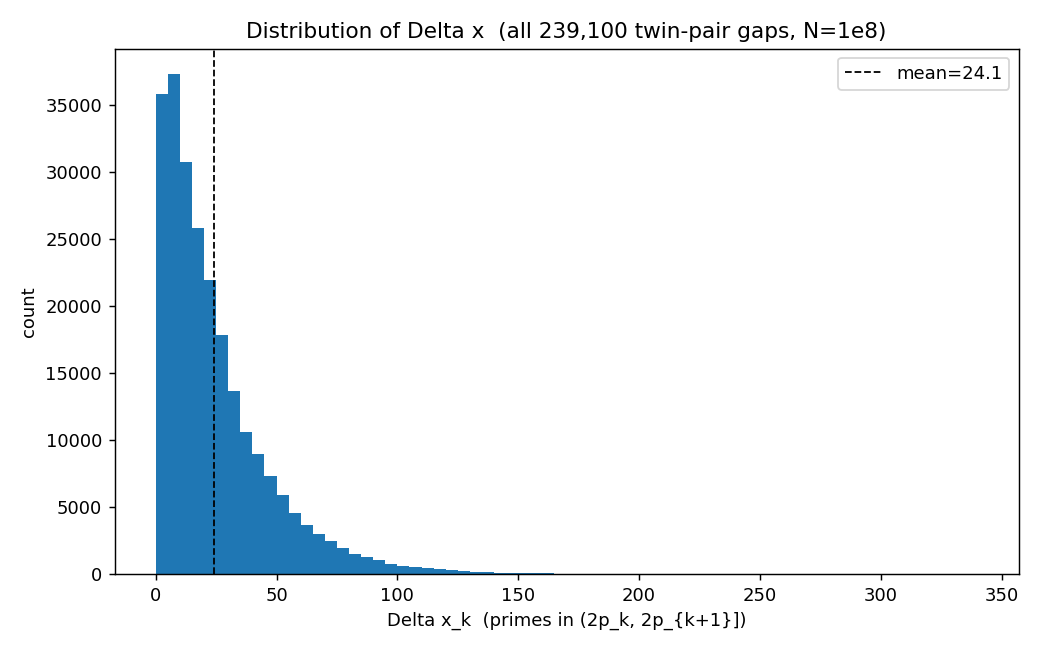
\includegraphics[width=0.8\textwidth]{deltax_histogram}
\caption{Distribution of $\Delta x_k$ over all $239\,100$ twin-pair gaps
(bins of width $5$; dashed line at the mean $24.1$). Mode in $[10,20)$, a
spike at $\Delta x=0$, and a thin right tail to $332$.}
\label{fig:deltax-hist}
\end{figure}

\subsection{The slope-drift law}\label{sec:deltax-slope}

By \eqref{eq:slope} the macro-slope of the shadow over a block of pairs is the
aggregate $1/\overline{\Delta x}$. (The per-step average
$\mathrm{mean}(1/\Delta x)$ is inadmissible: it is undefined on the $3\,819$
zero windows and Jensen-biased otherwise.) Differentiating the densities,
\[
   \mathrm{slope}
   =\frac{dk}{d\pi(2T)}
   =\frac{2C_2/(\log T)^2}{2/\log(2T)}
   =\frac{C_2\,\log(2T)}{(\log T)^2},
\tag{$\ast\ast$}\label{eq:slope-theory}
\]
whose leading coefficient is exactly $C_2=C_H/2$, half the Factor-Skyline
twin constant $C_H=2C_2$ established in Theorem~4.7a of the Factor Skyline
foundation paper~\cite{FS1}. Equation~\eqref{eq:slope-theory} exceeds the
crude $C_2/\log(2T)$ by the factor $(\log(2T)/\log T)^2\approx 1.1$.
Table~\ref{tab:deltax-slope} confirms~\eqref{eq:slope-theory} to $1$--$2\%$
across five decades.

\begin{table}[h]
\centering
\caption{Decade slope drift of the doubled-twin shadow. Empirical aggregate
slope $1/\overline{\Delta x}$ versus the refined prediction
$C_2\log(2T)/(\log T)^2$.}\label{tab:deltax-slope}
\begin{tabular}{lrrrr}
\toprule
decade of $T_k$ & $N$ & $\overline{\Delta x}$ & emp.\ slope & ratio to \eqref{eq:slope-theory} \\
\midrule
$[10^2,10^3)$        & $27$       & $9.70$  & $0.10305$ & $0.809$ \\
$[10^3,10^4)$        & $170$      & $11.50$ & $0.08696$ & $1.009$ \\
$[10^4,10^5)$        & $1\,019$   & $15.45$ & $0.06471$ & $0.982$ \\
$[10^5,10^6)$        & $6\,945$   & $18.85$ & $0.05304$ & $0.990$ \\
$[10^6,10^7)$        & $50\,811$  & $22.08$ & $0.04530$ & $1.004$ \\
$[10^7,5\cdot10^7)$  & $180\,120$ & $24.93$ & $0.04011$ & $0.998$ \\
\bottomrule
\end{tabular}
\end{table}

The slope drifts monotonically downward, $0.103\to0.040$, exactly the $1/\log$
behavior; the first decade $[10^2,10^3)$ is the sole outlier, in the
non-asymptotic regime. A free two-term fit
$\mathrm{slope}\approx A/L+B/L^2$ in $L=\log(2T)$ gives $A=0.795$, $B=-0.653$;
the apparent excess of $A$ over $C_2$ is an artifact of the bare
parametrization (expanding \eqref{eq:slope-theory} in $L$ gives
$A=C_2=0.660$, $B=2C_2\log2=0.915$), and the direct comparison of
Table~\ref{tab:deltax-slope} is the robust statement. Figure~\ref{fig:slope}
shows the decade points threading the backbone~\eqref{eq:slope-theory}.

\begin{figure}[h]
\centering
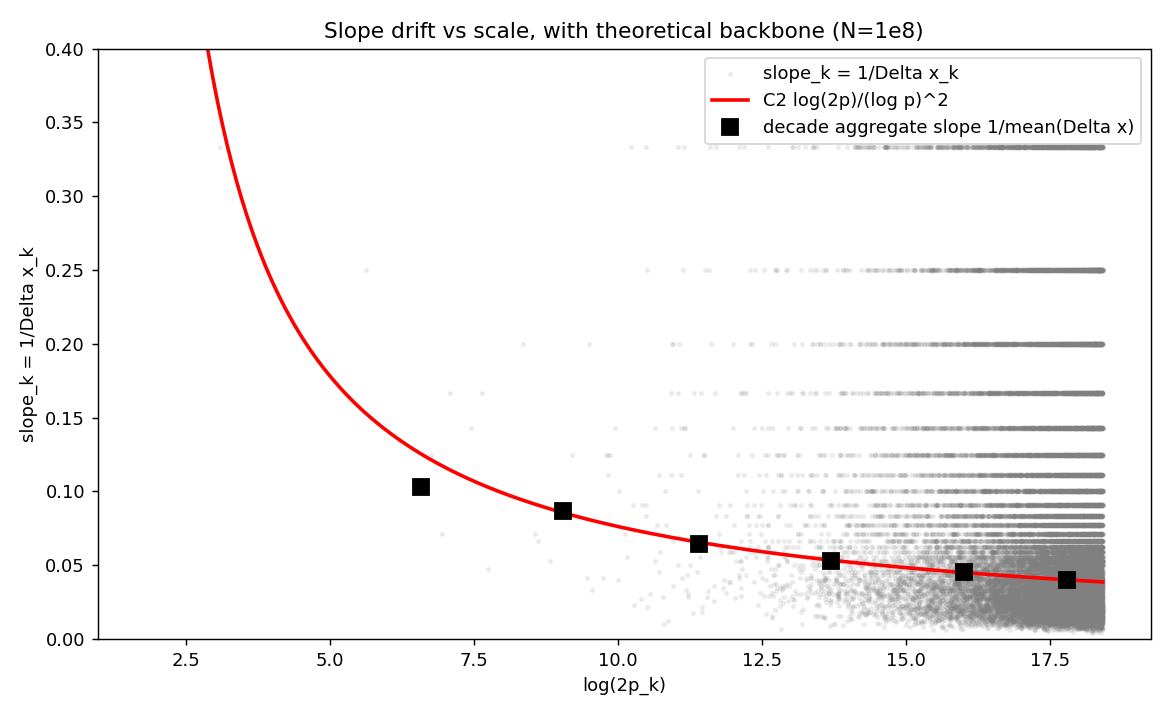
\includegraphics[width=0.85\textwidth]{slope_vs_log2p}
\caption{Local slope $1/\Delta x_k$ (gray, $30\,000$-point subsample) versus
$\log(2T_k)$, with the backbone $C_2\log(2T)/(\log T)^2$ (red) and the six
decade-aggregate slopes (squares). The discrete stripes are the admissible
values $1,\tfrac12,\tfrac13,\dots$ of $1/\Delta x$.}
\label{fig:slope}
\end{figure}

\subsection{Variance decomposition: the twin gap dominates}\label{sec:deltax-var}

Write the window length as $2G_k$, where $G_k=T_{k+1}-T_k$ is the twin gap of
Section~\ref{sec:empirical}, and define the local-density estimator
$\widehat\lambda_k=\Delta x_k/(2G_k)$, so that
\[
   \Delta x_k = 2G_k\cdot\widehat\lambda_k,\qquad
   \log\Delta x_k=\log(2G_k)+\log\widehat\lambda_k.
\]
The estimator $\widehat\lambda_k$ tracks the prime number theorem value
$\lambda_k=1/\log(2T_k)$ closely: the ratio
$r_k=\widehat\lambda_k/\lambda_k$ has mean $0.992$, median $0.995$, and
standard deviation $0.285$ (Figure~\ref{fig:scatter}). Partitioning the
log-variance,
\[
   \mathrm{Var}(\log\Delta x)=1.122,\quad
   \mathrm{Var}(\log 2G)=1.142,\quad
   \mathrm{Var}(\log\widehat\lambda)=0.076,
\]
the width term alone accounts for essentially the entire variance (the
density term is cancelled by a negative covariance). Equivalently, the
coefficients of variation are $0.955$ for $\Delta x$ and $0.953$ for $G$, but
only $0.300$ for $\widehat\lambda$.

\begin{proposition}\label{prop:deltax-var}
The fluctuations of $\Delta x_k$ are inherited essentially entirely from the
twin-gap sequence $G_k$, not from the local prime density: the
density factor $\widehat\lambda_k$ is rigid (it hugs $1/\log(2T)$ with
$\pm 29\%$ scatter), whereas $G_k$ is heavy-tailed (range $2$ to $2\,832$,
coefficient of variation $0.95$).
\end{proposition}

In particular the slope identity~\eqref{eq:slope} factors as
$\mathrm{slope}_k\approx\log(2T_k)/(2G_k)$: the slowly growing
$\log(2T_k)$ is the deterministic drift of Table~\ref{tab:deltax-slope},
while $1/G_k$ is the noise. The twin-gap growth law of
Section~\ref{sec:empirical} therefore governs the scatter of the doubled-twin
shadow directly.

\begin{figure}[h]
\centering
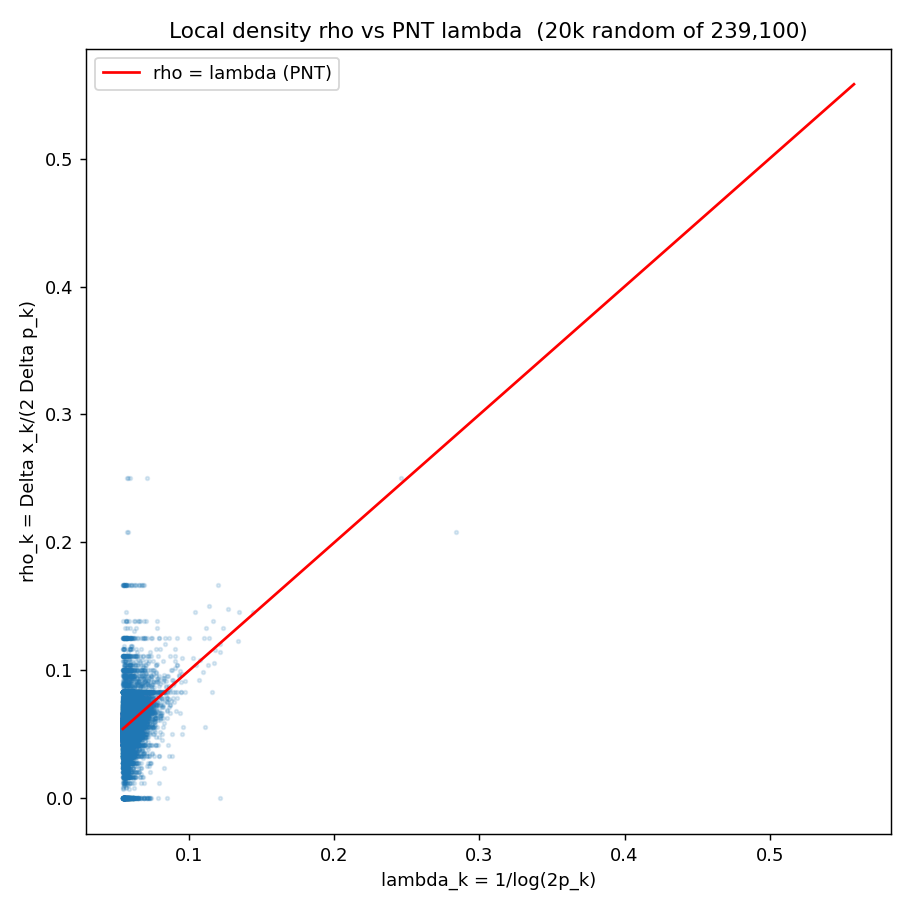
\includegraphics[width=0.7\textwidth]{lambda_rho_scatter}
\caption{Local density $\widehat\lambda_k=\Delta x_k/(2G_k)$ versus the PNT
prediction $\lambda_k=1/\log(2T_k)$ ($20\,000$-point subsample), with the
diagonal $\widehat\lambda=\lambda$. The cloud is centered on the diagonal
(mean ratio $0.99$) with bounded $\pm 29\%$ spread.}
\label{fig:scatter}
\end{figure}

\subsection{A Poisson-mixture model and the chance nature of collinearity}\label{sec:deltax-poisson}

The linearity of the shadow invites the question whether three or more
consecutive points are ever exactly collinear. By~\eqref{eq:slope} this asks
whether $\Delta x_k=\Delta x_{k+1}$. Empirically, equal adjacent gaps occur in
only $1.95\%$ of positions; the longest exact straight run in $239\,100$ gaps
is six points, occurring once. So collinearity beyond pairs is rare and
unstructured.

This rate is precisely what chance predicts. Modeling the primes near $2T_k$
as an inhomogeneous Poisson process of intensity $1/\log t$, the count
$\Delta x_k$ is Poisson with mean
$\mu_k\approx 2G_k/\log(2T_k)$; since $G_k$ varies widely, the marginal of
$\Delta x$ is a \emph{Poisson mixture}, strongly overdispersed (variance
$529.8$ against mean $24.10$, ratio $\approx 22$). For independent draws from
the empirical marginal, the expected coincidence rate is
$\sum_v\Pr[\Delta x=v]^2=1.99\%$, matching the observed $1.95\%$; a single
Poisson of the same mean would predict $5.76\%$, far too high because it is
too concentrated. Hence the collinearity rate carries no signal: it is the
chance coincidence rate of an overdispersed, twin-gap-driven gap process. (This
overdispersion is the gap-count companion of the extreme-gap overshoot
documented in Section~\ref{sec:empirical}.)

\subsection{Scale-collapse of the conditional gap}\label{sec:deltax-collapse}

Normalizing by the full conditional mean, set $Z_k=\Delta x_k/\mu_k$ with
$\mu_k=2G_k/\log(2T_k)$; algebraically $Z_k=r_k$ of
Section~\ref{sec:deltax-var}. Binning by decades of $T_k$, the distribution of
$Z_k$ collapses onto a single scale-invariant shape: it is unimodal, centered
just below $1$, with standard deviation $\approx 0.28$ at every scale, and the
Kolmogorov--Smirnov distance between decades falls to $0.021$ between the two
largest (Table~\ref{tab:deltax-collapse}).

\begin{table}[h]
\centering
\caption{Scale-collapse of $Z_k=\Delta x_k/\mu_k$. The KS column is the
distance to the next decade.}\label{tab:deltax-collapse}
\begin{tabular}{lrrrr}
\toprule
decade of $T_k$ & $N$ & $\overline{Z}$ & $\mathrm{std}\,Z$ & KS to next \\
\midrule
$[10^2,10^3)$        & $27$       & $0.940$ & $0.256$ & $0.166$ \\
$[10^3,10^4)$        & $170$      & $0.956$ & $0.277$ & $0.071$ \\
$[10^4,10^5)$        & $1\,019$   & $0.976$ & $0.256$ & $0.063$ \\
$[10^5,10^6)$        & $6\,945$   & $0.991$ & $0.290$ & $0.026$ \\
$[10^6,10^7)$        & $50\,811$  & $0.992$ & $0.288$ & $0.021$ \\
$[10^7,5\cdot10^7)$  & $180\,120$ & $0.993$ & $0.284$ & --- \\
\bottomrule
\end{tabular}
\end{table}

The normalization removes the twin-gap-driven overdispersion entirely: the
coefficient of variation falls from $0.955$ for $\Delta x$ to $0.287$ for $Z$,
and is scale-stable. What remains is \emph{not} pure Poisson shot noise: a
Poisson model predicts $\mathrm{std}\,Z\approx1/\sqrt{\overline{\Delta x}}$,
which would fall through $0.32,0.30,0.25,0.23,0.21,0.20$ across the six
decades, whereas the observed spread holds near $0.28$ and increasingly
exceeds the Poisson reference. The conditional gap is thus mildly
super-Poissonian, consistent with the excess variance of primes in short
intervals~\cite{MS2004}, and the residual is a genuine, scale-free arithmetic
fluctuation.

\subsection{Synthesis}\label{sec:deltax-synth}

The doubled-twin shadow decomposes cleanly: a deterministic $1/\log$ slope
drift (Table~\ref{tab:deltax-slope}, leading constant $C_2=C_H/2$) carrying
twin-gap-driven, scale-free counting noise
(Proposition~\ref{prop:deltax-var}, Section~\ref{sec:deltax-collapse}). The
three successive normalizations form a ladder of decreasing variability,
$\Delta x\ (\mathrm{CV}=0.955)\to\widehat\lambda\ (0.300)\to Z\ (0.287)$, each
peeling away one structural layer (window width, then density trend) until
only the irreducible arithmetic fluctuation remains.

In the Factor-Skyline reading that motivates $(\mathrm{TPB})$ (the
coverage/escape architecture of~\cite{FS1}), this is exactly the split between
what the coverage template supplies for free and what the escape layer cannot:
the
candidate windows and their density --- the deterministic backbone above ---
are template structure, governed by the same constant $C_H$ that
Theorem~4.7a~\cite{FS1} identifies with the Hardy--Littlewood singular series,
while the scale-free residual $Z$ is the escape randomness. The geometry of
doubled twins thus renders the $(\mathrm{TPB})$ density mechanism visible: a
predictable trend that guarantees candidates, dressed in a fluctuation that no
coverage argument controls.

\section{Twin-Ramanujan Primes and the Dyadic Twin-Prime Threshold}
\label{sec:twin-ramanujan}

The $(\mathrm{TPB})$ inequality $\pi_2(2x)-\pi_2(x)\ge 1$ asks for
\emph{at least one} twin prime in every dyadic window past a cutoff.
A natural strengthening is to ask for \emph{at least $n$} twin primes
in every dyadic window. This yields a family of thresholds in direct
analogy with the classical Ramanujan primes.

\subsection{Classical Ramanujan primes}

Ramanujan~\cite{Ramanujan1919} proved that for every integer $n\ge 1$,
the inequality $\pi(x)-\pi(x/2)\ge n$ holds for all sufficiently large
$x$. The $n$-th Ramanujan prime is defined as
\begin{equation}\label{eq:R-classical}
R_n \;=\; \min\Big\{\,R\,:\,\pi(x)-\pi(x/2)\ge n\ \text{for all}\ x\ge R\,\Big\},
\end{equation}
so that $R_1=2$ (Bertrand's postulate itself). The first several values are
$R_n=2,\,11,\,17,\,29,\,41,\,59,\,67,\,71,\ldots$
(OEIS \texttt{A104272}~\cite{OEIS_A104272}). Sondow~\cite{Sondow2009}
established the asymptotic $R_n\sim p_{2n}$ (twice the $n$-th prime)
and initiated the modern study of this sequence; later work extended
the construction to $c$-Ramanujan primes and related
objects~\cite{Amersi2014,Paksoy2012}.

\subsection{The twin analog}

We define, in direct parallel,
\begin{equation}\label{eq:R-twin}
R^{\mathrm{twin}}_n \;=\; \min\Big\{\,R\,:\,\pi_2(x)-\pi_2(x/2)\ge n\ \text{for all}\ x\ge R\,\Big\},
\end{equation}
the least cutoff past which every dyadic interval $(x/2,x]$ contains
at least $n$ twin primes. By construction, $R^{\mathrm{twin}}_n$ is
non-decreasing in $n$, and $(\mathrm{TPB})$ is exactly the statement
that $R^{\mathrm{twin}}_1$ exists and is equal to $11$.

\begin{theorem}\label{thm:R1}
$R^{\mathrm{twin}}_1 = 11$.
\end{theorem}

\begin{proof}[Proof (restatement of $(\mathrm{TPB})$ verification)]
The function $f(x) := \pi_2(x) - \pi_2(x/2)$ is piecewise constant with
a $+1$ jump at each twin prime $x = T_k$ and a $-1$ jump at each
$x = 2T_k$. Direct evaluation on the first few twins shows $f(x) = 0$
on $[10,11)$ (because $\pi_2(10) = 2$ and $\pi_2(5) = 2$), whereas
$f(11) = \pi_2(11) - \pi_2(5.5) = 3 - 2 = 1$. A finite check for
$x\in[11,1000]$ confirms $f(x)\ge 1$ throughout, and the verification
of $(\mathrm{TPB})$ for $x\le 10^{10}$ in Section~\ref{sec:empirical}
extends this to all tested $x$. Hence the infimum in~\eqref{eq:R-twin}
with $n=1$ is $11$.
\end{proof}

\subsection{Computed values}

From the twin-prime list up to $10^{10}$, we computed $R^{\mathrm{twin}}_n$
via an event walk on the $42$ million $\pm 1$ transitions of $f$.
Every $R^{\mathrm{twin}}_n$ lies within the data-certified range when
$n\le f(10^{10}) = 12{,}794{,}513$. Because $f$ at the top of our range
exceeds this maximum $n$ by construction, each computed value is a
true threshold, not merely an upper bound.

\begin{table}[h]
\centering
\caption{First 30 twin-Ramanujan primes.}\label{tab:R-first}
\begin{tabular}{rr|rr|rr}
\toprule
$n$ & $R^{\mathrm{twin}}_n$ & $n$ & $R^{\mathrm{twin}}_n$ & $n$ & $R^{\mathrm{twin}}_n$ \\
\midrule
1 & 11 & 11 & 821 & 21 & 1787 \\
2 & 59 & 12 & 1019 & 22 & 1871 \\
3 & 101 & 13 & 1049 & 23 & 1877 \\
4 & 149 & 14 & 1061 & 24 & 1931 \\
5 & 179 & 15 & 1289 & 25 & 1949 \\
6 & 227 & 16 & 1319 & 26 & 2081 \\
7 & 569 & 17 & 1427 & 27 & 2129 \\
8 & 599 & 18 & 1451 & 28 & 2237 \\
9 & 641 & 19 & 1481 & 29 & 2657 \\
10 & 809 & 20 & 1667 & 30 & 2687 \\
\bottomrule
\end{tabular}
\end{table}

\begin{table}[h]
\centering
\caption{Larger $R^{\mathrm{twin}}_n$ at logarithmic scales.}\label{tab:R-log}
\begin{tabular}{rr}
\toprule
$n$ & $R^{\mathrm{twin}}_n$ \\
\midrule
$100$           & $14{,}009$ \\
$1\,000$        & $217{,}337$ \\
$10\,000$       & $3{,}241{,}487$ \\
$100\,000$      & $45{,}529{,}751$ \\
$1\,000\,000$   & computed in \texttt{data/twin\_ramanujan\_primes.csv} \\
\bottomrule
\end{tabular}
\end{table}

\begin{remark}[Every $R^{\mathrm{twin}}_n$ is a twin prime]
\label{rem:R-is-twin}
The function $f$ changes by $\pm 1$ at isolated events: $+1$ at each
twin prime $T_k$ and $-1$ at each $x = 2T_k$. A transition of $f$
from strictly below $n$ to at least $n$ can only occur at a $+1$
event, i.e., at a twin prime. Since $R^{\mathrm{twin}}_n$ is defined
as the smallest $R$ past which $f\ge n$ is sustained, it coincides
with the first twin prime at which such a sustained transition is
achieved. In particular, every $R^{\mathrm{twin}}_n$ is itself a twin
prime. We verified this directly for all $n\le 10^6$ in our data: all
one million computed values are twin primes.
\end{remark}

\subsection{Growth rate}

Sondow's asymptotic for the classical sequence is
\begin{equation}\label{eq:R-asymp-classical}
R_n \;\sim\; p_{2n} \;\sim\; 2n\log n
\qquad(n\to\infty).
\end{equation}
The heuristic analog for twins comes directly from the
Hardy--Littlewood prediction
$\pi_2(x)\sim 2C_2\,x/(\log x)^2$: writing
$R=R^{\mathrm{twin}}_n$ and requiring
$\pi_2(R)-\pi_2(R/2)\approx n$, we obtain
$n\approx 2C_2\,R/(2(\log R)^2)$, hence
\begin{equation}\label{eq:R-asymp-twin}
R^{\mathrm{twin}}_n \;\sim\; \frac{n\,(\log n)^2}{C_2} \qquad(n\to\infty),
\end{equation}
a factor of roughly $\log n /(2C_2) \approx 0.76\log n$ times the
ordinary $R_n$. On the data range considered here, the observed ratio
$R^{\mathrm{twin}}_n / R_n$ grows slowly with $n$, consistent
with~\eqref{eq:R-asymp-twin} up to the finite-size corrections
documented in Section~\ref{sec:empirical}.

\subsection{Positioning}

Theorem~\ref{thm:R1} recasts $(\mathrm{TPB})$ as the statement
$R^{\mathrm{twin}}_1 = 11$, placing it inside the
Ramanujan-prime family of dyadic-density thresholds. The classical
Ramanujan primes quantify how large $x$ must be before every dyadic
interval contains $n$ \emph{ordinary} primes; the twin-Ramanujan
primes ask the same question for twin primes. The construction is
the immediate analog of Ramanujan's original definition, but replaces
$\pi$ by $\pi_2$; $c$-Ramanujan primes~\cite{Amersi2014} generalize
in a different direction (varying the interval ratio $c$ for the
ordinary-prime count). To our knowledge, the specific sequence
$R^{\mathrm{twin}}_n$ has not previously been defined or tabulated;
we propose it as the natural dyadic-density sequence attached to
twin primes, and the corresponding data file (first $10^6$ values)
as a candidate for inclusion in the OEIS.

The same construction applies to any admissible pair-constellation
$\mathcal{C} = \{0, g\}$, yielding $R^{\mathcal{C}}_n$. The first
values for $\mathcal{C} \in \{\{0,4\},\{0,6\}\}$ are
$R^{\{0,4\}}_1 = 7$ and $R^{\{0,6\}}_1 = 5$, giving the cousin and
sexy thresholds a geometric interpretation; this is developed in
PG~III as the Generalized Bertrand Principle.

\section{Related Work}\label{sec:lit}

The study of twin primes is extensive. We summarize the most directly
relevant strands.

\paragraph{Ramanujan primes.}
Ramanujan's 1919 theorem~\cite{Ramanujan1919} that
$\pi(x)-\pi(x/2)\ge n$ holds for all $x\ge R_n$ is the direct parent
of $(\mathrm{TPB})$. Sondow~\cite{Sondow2009} modernized the theory
with the asymptotic $R_n\sim p_{2n}$;
Amersi--Beckwith--Miller--Ronan--Sondow~\cite{Amersi2014}
generalized to $c$-Ramanujan primes (varying the interval ratio), and
Paksoy~\cite{Paksoy2012} introduced derived Ramanujan primes.
Sondow--Nicholson--Noe~\cite{SondowNicholsonNoe2011} studied which
Ramanujan primes happen to be twin primes (a different object from
our $R^{\mathrm{twin}}_n$: they examine ordinary Ramanujan primes
that fall within twin-prime pairs, whereas $R^{\mathrm{twin}}_n$ is
the dyadic-density threshold for $\pi_2$ itself).

\paragraph{The Hardy--Littlewood conjecture.}
Hardy and Littlewood conjectured in 1923 that the number of twin
primes up to $x$ is asymptotically
$2C_2\int_2^x dt/(\log t)^2$, with $C_2$ the twin-prime constant. No
non-trivial lower bound of this form, or even of the form
$\pi_2(x)\gg x/(\log x)^A$, is known unconditionally.

\paragraph{Bounded gaps.}
Zhang's 2013 theorem established that
$\liminf_{n\to\infty}(p_{n+1}-p_n)<\infty$ with a bound of
$7\times 10^7$. The Polymath8 collaboration reduced this to $4\,680$
using refinements of Zhang's method, and to $246$ using Maynard's
multi-variable sieve (Polymath8b). Under the Elliott--Halberstam
conjecture, the bound drops to $12$, and under the generalized
Elliott--Halberstam conjecture it reaches $6$. None of these results
give a twin prime (gap $2$) in \emph{every} interval $(x,2x]$; they
give a bounded-gap pair at \emph{some} scales infinitely often.

\paragraph{Explicit bounds on $\pi_2$.}
Upper bounds of Brun-sieve and Selberg-sieve type give
$\pi_2(x)\ll x/(\log x)^2$ unconditionally, which is compatible with
HL up to a constant factor. Explicit constants are known in the sieve
literature; they are not sharp enough to yield $(\mathrm{TPB})$
unconditionally in any finite range beyond direct computation.

\paragraph{Twin primes in short intervals.}
Classical results (Heath-Brown, Friedlander-Iwaniec, and others)
give conditional short-interval estimates of the form
$\pi_2(x+y)-\pi_2(x)>0$ for $y\ge x^{1-\delta}$ under various
hypotheses; however these do not reduce $y$ to $x$ (the dyadic scale)
unconditionally. We are not aware of a statement in the literature
that isolates the dyadic inequality $\pi_2(2x)\ge\pi_2(x)+1$ as a
target in its own right.

\paragraph{Summary.}
$(\mathrm{TPB})$ occupies a gap in the literature: it is natural,
elementary to state, verifiable by direct computation, and believed
true, yet it has not been articulated explicitly as a conjecture.
Its provability under Hardy--Littlewood is immediate; its
unconditional proof appears to require either a stronger
short-interval result than is currently available or a new
sieve-theoretic input.

\section{Conclusion}

$(\mathrm{TPB})$ is a clean, elementary, unproven conjecture about
twin primes that sits strictly between the Zhang--Maynard
bounded-gaps theorems and the full twin-prime conjecture. It is
equivalent to the ratio statement $T_{k+1}<2T_k$ for $T_k\ge 11$,
equivalent to the geometric statement that every angle-record
of the Prime Triangle sequence with $p_n\ge 3$ is a twin prime,
and equivalent to the identity $R^{\mathrm{twin}}_1=11$ within the
Ramanujan-prime family.

The four formulations are mutually reducible via the elementary
$2P$-beats lemma and the Ramanujan-threshold construction; each
provides a different avenue for verification and potential proof.
Our computations verify $(\mathrm{TPB})$ for all $x\le 10^9$, a range
that dwarfs the scales at which the ratio envelope tightens to
$r_k<1.001$, and produce the twin-Ramanujan sequence
$R^{\mathrm{twin}}_n$ for $n$ up to $12\,794\,513$.

We have also observed that the average twin-gap is well-fitted by
$0.70(\log T_k)^{1.866}$ and that the extreme-gap overshoot
$\max G_k/(\log T_k)^2$ grows monotonically across decades. Whether
the exponent $\beta$ converges to $2$ asymptotically, and whether the
overshoot growth follows a $(\log\log T)$ or power-of-$\log\log T$
law, are open empirical questions.

A near-term goal is the unconditional proof of $(\mathrm{TPB})$ by a
sieve-theoretic argument adapting the Maynard multi-dimensional
sieve to the dyadic short-interval regime; a complementary goal is
the extension of the empirical verification to $10^{12}$ and beyond.
We leave both to future work.

\section*{Data availability}

All computations reproduce from
\texttt{scripts/pg\_twin\_angle\_analysis.py} and
\texttt{scripts/pg\_twin\_ramanujan.py}. The derived datasets
(\texttt{twins\_1e9.npy}, \texttt{twins\_1e10.npy},
\texttt{angle\_records\_1e8.csv}, \texttt{ratio\_top20.csv},
\texttt{decade\_gap\_table.csv},
\texttt{twin\_ramanujan\_primes.csv}) are stored alongside.

\section*{Acknowledgements}

This paper builds on PG~I (\emph{The Prime Triangle and its
Geometric Invariants}, Proxmire, April 2026) and the PSD Factor note
(\emph{Prime Triangles and the Prime Square-Difference Identity},
Proxmire, November 2025). The Ramanujan-prime context grew out of a
literature search performed in April 2026.

\begin{thebibliography}{99}

\bibitem{Ramanujan1919}
S.~Ramanujan.
\emph{A proof of Bertrand's postulate}.
J.~Indian Math.\ Soc.\ \textbf{11} (1919), 181--182.

\bibitem{Sondow2009}
J.~Sondow.
\emph{Ramanujan primes and Bertrand's postulate}.
Amer.\ Math.\ Monthly \textbf{116} (2009), 630--635.
arXiv:\href{https://arxiv.org/abs/0907.5232}{0907.5232}.

\bibitem{SondowNicholsonNoe2011}
J.~Sondow, J.~W.~Nicholson, T.~D.~Noe.
\emph{Ramanujan primes: bounds, runs, twins, and gaps}.
J.~Integer Seq.\ \textbf{14} (2011), Article 11.6.2.
arXiv:\href{https://arxiv.org/abs/1105.2249}{1105.2249}.

\bibitem{Amersi2014}
N.~Amersi, O.~Beckwith, S.~J.~Miller, R.~Ronan, J.~Sondow.
\emph{Generalized Ramanujan primes}.
In: \emph{Combinatorial and Additive Number Theory~--- CANT 2011 and 2012},
Springer Proc.\ Math.\ Stat.\ \textbf{101} (2014), 1--13.

\bibitem{Paksoy2012}
M.~B.~Paksoy.
\emph{Derived Ramanujan primes: $R'_n$}.
arXiv:\href{https://arxiv.org/abs/1210.6991}{1210.6991} (2012).

\bibitem{OEIS_A104272}
OEIS Foundation Inc.
\emph{Entry A104272: Ramanujan primes}.
Online at \url{https://oeis.org/A104272}.

\bibitem{FS1}
A.~Proxmire.
\emph{The Factor Skyline: An Ontological Lookout Over the Integers}.
Zenodo, 2026.
DOI:\,\href{https://doi.org/10.5281/zenodo.18275273}{10.5281/zenodo.18275273}.
(Architectural Foundation, \S4.3.1, Theorem~4.7a: the twin coverage constant
$C_H=2C_2$.)

\bibitem{MS2004}
H.~L.~Montgomery, K.~Soundararajan.
\emph{Primes in short intervals}.
Comm.\ Math.\ Phys.\ \textbf{252} (2004), 589--617.

\end{thebibliography}

\end{document}
